\documentclass{article}[12pt]

%----- Math ---------------------------------------------
\usepackage{amsmath}   
\usepackage{mathrsfs}      
\usepackage{mathtools}       
\usepackage{amssymb}   
\usepackage{amsthm}   
\usepackage{esint}     
\usepackage{resmes} 
\usepackage{stackengine}
\usepackage{amsfonts}
\usepackage{stmaryrd}
\usepackage{dsfont}



%----- Design ------------------------------------------- 
\usepackage{lastpage}                              
\usepackage{enumitem}
\usepackage{multirow}


%----- Intestazioni ---------------------------------------
\usepackage{fancyhdr}
\pagestyle{fancy}
\fancyhf{} % Clear all headers and footers
\fancyhead[R]{\nouppercase{\leftmark}} % Header right on all pages
\fancyfoot[C]{\thepage} % Footer center, page number
\setlength{\headheight}{14.5pt}

% Pacchetto titlesec per personalizzare i titoli dei capitoli
\usepackage{titlesec}


%----- Pacchetti Disegno --------------------------------
\usepackage{tikz}
\makeatother 
\usetikzlibrary{3d,perspective}
\usetikzlibrary{patterns}
\usetikzlibrary{arrows,calc,patterns}
\usepackage{tikz-cd}
\usepackage{graphicx}
\usepackage{thmtools}
\usepackage{xcolor}
\usepackage[all]{xy}        
\usetikzlibrary{decorations.markings}
\usetikzlibrary{hobby}
\usepackage{pgfplots}
\pgfplotsset{compat=1.18}


%----- Symbols -----------------------------------------
\input{symbols}

%----- Hyperref ------------------------------------------
\usepackage{nameref}
\usepackage{csquotes}
\usepackage{hyperref}
\hypersetup{
	colorlinks=true,
	linkcolor=black, % Color for normal internal links
	filecolor=black, % Color for file links
	urlcolor=blue, % Color for external links
	citecolor=blue % Color for citations
}
\usepackage{cleveref} 


% -----Ambienti matematici-------------------------------
\theoremstyle{plain}
\newtheorem{thm}{Theorem}[section]
\newtheorem*{thm*}{Theorem}
\newtheorem{prop}[thm]{Proposition}
\newtheorem{cor}[thm]{Corollary}
\newtheorem{lemma}[thm]{Lemma}
\newtheorem{claim}{Claim}
\newtheorem{pbm}{Problem}

\theoremstyle{definition}
\newtheorem{defn}[thm]{Definition}
\newtheorem{axiom}{Axiom}

\theoremstyle{remark}
\newtheorem{rmk}[thm]{Remark}
\newtheorem{ex}[thm]{Example}
\newtheorem{exercise}{Exercise}


%------BIBLIOGRAFIA-----------
\usepackage[style=alphabetic, maxbibnames=4, minbibnames=4, giveninits=true]{biblatex}
\ExecuteBibliographyOptions{
      maxalphanames = 4,
      maxcitenames  = 3,
      minalphanames = 3,
      minnames      = 1
    }
% Definizione di un nuovo driver per nascondere URL e DOI
\AtEveryBibitem{
	\clearfield{url} 
    \clearfield{doi} 
    \clearfield{isbn} 
    \clearfield{issn} 
    \clearfield{note} 
    %\clearfield{archivePrefix} 
    \clearfield{eprint} 
    \clearfield{urldate}
    \clearfield{urlyear}
    \clearfield{urlmonth}
    \clearfield{urlday}
    \clearfield{address}
}
\addbibresource{biblio.bib}

\title{Bernstein problem}
\author{Andrea Martelli}
\date{February 2026}

\begin{document}

\maketitle
\tableofcontents


\section{Introduction and history}
Let \(\Sigma \subset \R^{n+1}\) be a two-sided, connected, embedded hypersurface, and fix a unit normal vector field \(\nu \colon \Sigma \to \Sp^n\). Recall that, since \(\R^{n+1}\) is simply connected, if \(\Sigma\) is also complete (equivalently, without boundary and embedded as closed subset) then \(\Sigma\) is orientable and two-sided. Since \(T_x\Sigma= T_{\nu(x)}\Sp^n\) as subspaces of \(\R^{n+1}\) for every \(x \in \Sigma\), the differential \(\dif \nu_x \colon T_x\Sigma \to T_x\Sigma \) is an endomorphism of \(T_x\Sigma\), called \emph{shape operator}. The bilinear form
\[
    A_\Sigma(X,Y) \coloneq -X \cdot \dif \nu(Y)
\]
is the \emph{second fundamental form} of \(\Sigma\). Its trace \(H_\Sigma\) is the mean curvature of \(\Sigma\).

\begin{thm}[First variation formula]
For every \(\vp \in C^\infty_c(\Sigma)\), let \(\Sigma_t \coloneq \{ x+t\vp(x)\nu(x) \colon x \in \Sigma\}\). 
Then
\begin{equation}
    \left.\frac{\dif}{\dif t}\right|_{t=0}\Haus^n(\Sigma_t) = \int_\Sigma H_\Sigma\vp \ \dif \Haus^n.
\end{equation}
\end{thm}

Thus \(\Sigma\) is a minimal hypersurface (i.e. stationary for the \(n\)-area functional) if and only if \(H \equiv 0\). 

If \(u \colon \Omega \subset \R^n \to \R\) is a smooth function, the mean curvature of its graph is
\[
    H_{\gr(u)} = \dive \left( \frac{\nabla u}{\sqrt{1+|\nabla u|^2}} \right)
\]
so \(\gr(u)\) is a minimal surface if and only if \(u\) solves
\begin{equation}\label{eq: MSE}
    \dive \left( \frac{\nabla u}{\sqrt{1+|\nabla u|^2}} \right) = 0. \tag{MSE}
\end{equation}


\begin{pbm}[Bernstein]
    Is every \emph{entire} solution \(u \colon \R^n \to \R\) of \eqref{eq: MSE} always affine?
\end{pbm}

This is a rigidity problem of a non linear PDE, like Liouville's theorem for harmonic functions. However, the non-linearity makes the answer quite a surprise. 
\begin{thm}\label{thm: solution of Bernstein problem}
    If \(n\le 7\), every entire solution \(u \colon \R^n \to \R\) of \eqref{eq: MSE} is affine.

    If \(n \ge 8\), there exists a non-affine entire solution \(u \colon \R^n \to \R\) of \eqref{eq: MSE}.
\end{thm}
This result has been proved by Bernstein \cite{Bernstein1927} for \(n=2\), De Giorgi \cite{DeGiorgi_EstensioneBernstein1965} for \(n=3\), Almgren \cite{Almgren_InteriorRegularity} for \(n=4\), Simons \cite{Simons_MinimalVarieties1968} for \(5\le n\le 7\), and by Bombieri, De Giorgi and Giusti \cite{BombieriDeGiorgiGiusti_MinimalCones1969} for \(n\ge 8\).

\section{Area minimizing hypersurfaces}
\begin{defn} 
We say that \(\Sigma\) is \emph{area minimizing} if every compact piece of \(\Sigma\) with smooth boundary minimizes the \(n\)-area among all other hypersurfaces with same boundary. In other words, \(\Sigma\) is area minimizing if for each compact set \(K \subset \R^{n+1}\) such that \(\Sigma \cap K\) is a smooth compact hypersurface with smooth boundary, then for every other compact hypersurface \(\Sigma'\) with \(\de \Sigma' = \de(\Sigma \cap K)\) we have
\[
    \Haus^n(\Sigma \cap K) \le \Haus^n(\Sigma')
\]
\end{defn}

A sufficient condition for being area minimizing is being \emph{calibrated}. 
\begin{defn}
    A calibration for \(\Sigma\) is a smooth vector field \(v \colon \R^{n+1} \to \R^{n+1}\) such that
    \begin{itemize}
        \item \(|v|\le 1\) on \(\R^{n+1}\);
        \item \(v \cdot \nu =1 \) on \(\Sigma\);
        \item \(\dive v = 0\) on \(\R^{n+1}\).
    \end{itemize}
\end{defn}
In particular, for every compact hypersurface \(\Sigma'\) (which necessarily is two-sided)
\[
    \int_{\Sigma'} v \cdot \nu' \dif \Haus^n \le \Haus^n(\Sigma')
\]
for any unit normal vector field \(\nu' \colon \Sigma' \to \Sp^n\).
\begin{lemma}
    If \(\Sigma\) is calibrated then it's area minimizing.
\end{lemma}
\begin{proof}
    Let \(\de \Sigma' = \de(\Sigma \cap K)\). Since transversality is an open condition, we can assume that \(\Sigma'\) meets \(\Sigma\) transversely. Moreover, up to consider each piece individually, we may also assume that \(\Sigma'\) is on one side of \(\Sigma\). In this case, we can find an open domain \(\Omega \subset \subset \R^{n+1}\) such that \(\de\Omega= \Sigma' \cup (\Sigma \cap K)\). Then by the divergence theorem
    \[
        \Haus^n(\Sigma') -\Haus^n(\Sigma\cap K) \ge \int_{\Sigma'} v \cdot \nu' \dif \Haus^n - \int_{\Sigma \cap K} v \cdot \nu \dif \Haus^n  = \pm \int_\Omega \dive v \dif x= 0,
    \]
    as required.
\end{proof}

An entire minimal graph is always calibrated by
\[
    v = \frac{(-\nabla u,1)}{\sqrt{1+|\nabla u|^2}},
\]
so in particular it's area minimizing. 

We are going to use three important features of area minimizing hypersurfaces:
\begin{itemize}
    \item stability
    \item extrinsic volume growth estimate
    \item weak* closure.
\end{itemize}

\subsection{Stability}
\begin{defn}
    A minimal hypersurface is \emph{stable} if for every \(\vp \in C^\infty_c(\Sigma)\), letting \(\Sigma_t \coloneq \{ x+t\vp(x)\nu(x) \colon x \in \Sigma\}\),
    \[
        \left.\frac{\dif^2}{\dif t^2}\right|_{t=0} \Haus^n(\Sigma_t) \ge 0.
    \]
\end{defn}
\begin{thm}[Second variation formula]
    Let \(\Sigma \subset \R^n\) be a minimal hypersurface. For every \(\vp \in C^\infty_c(\Sigma)\), let \(\Sigma_t \coloneq \{ x+t\vp(x)\nu(x) \colon x \in \Sigma\}\). 
    Then
    \begin{equation}
        \left.\frac{\dif^2}{\dif t^2}\right|_{t=0}\Haus^n(\Sigma_t) = \int_\Sigma |\nabla_\Sigma\vp|^2-|A_\Sigma|^2\vp^2 \dif \Haus^n = - \int_\Sigma \vp L_\Sigma \vp \ \dif \Haus^n,
    \end{equation}
    where
    \[
        L_\Sigma = \Delta_\Sigma + |A_\Sigma|^2
    \]
    is the \emph{Jacobi operator} of \(\Sigma\).
\end{thm}

Therefore a minimal hypersurface \(\Sigma \subset \R^{n+1}\) is stable if and only if the \emph{stability inequality} holds
\begin{equation}\label{eq: stability inequality}
    \int_\Sigma |\nabla_\Sigma \vp|^2 - |A_\Sigma|^2\vp^2\dif \Haus^n \ge 0 \qquad \forall \vp \in C^\infty_c(\Sigma).
\end{equation}
Observe that, in particular, every area minimizing hypersurface is stable.

Since \(L_\Sigma\) is self-adjoint elliptic operator, setting homogeneous boundary conditions it can be diagonalized on every relatively compact domain \(\Omega \subset \subset \Sigma\), and the first eigenvalue can be characterized as
\[
    \lambda_1(\Omega) \coloneq \inf \left\{ \frac{\int_\Omega |\nabla_\Sigma \vp|^2 - |A_\Sigma|^2 \vp^2 \dif \Haus^n}{\int_\Omega \vp^2 \dif \Haus^n} \colon \vp \in C^\infty_c(\Omega) \setminus\{0\} \right\}.
\]
Therefore, \(\Sigma\) is stable if and only if
\[
    d_0(\Sigma) \coloneq \inf_{\Omega \subset \subset \Sigma} \lambda_1(\Omega) \ge 0.
\]

\subsection{Extrinsic volume growth estimate}
\begin{thm}\label{thm: quadratic area growth for entire minimal graphs}
	If \(\Sigma\) is a complete area minimizing hypersurface in \(\R^{n+1}\), then for all \(r>0\)
	\[
		\Haus^n(\gr(u) \cap B_r) \leq \frac{(n+1)\omega_{n+1}}{2} r^n
	\]
	where \(B_r=B_r(0)\) is the ball of \(\R^{n+1}\) centered at the origin with radius \(r\) and \((n+1)\omega_{n+1}\) is the \(\Haus^n\)-measure of the standard unit sphere \(\Sp^n \subset \R^{n+1}\).
\end{thm}
 
\begin{proof}
	By Sard's theorem the set of positive real numbers \(r>0\) such that \(\Sigma\) intersects \(S_r\coloneq \de B_r\) transversely is dense in \(\R_{>0}\), so we can prove the statement assuming that \(\Sigma\) intersects \(S_r\) transversely. Assume also that \(\Gamma \coloneq \Sigma \cap S_r \ne \varnothing\). The implicit function theorem implies that \(\Gamma\) is a (compact, but possibly non connected) \((n-1)\)-dimensional manifold without boundary. By Jordan-Brouwer separation theorem, each connected component \(\Gamma_j\) of \(\Gamma\) separates \(S_r\) into two connected components having boundary \(\Gamma_j\), and in this way we can write \(S_r \setminus \Gamma= \Sigma_1 \sqcup \Sigma_2\) with \(\Sigma_1, \Sigma_2\) having common boundary \(\Gamma\) (see Figure~\ref{fig: connected components}). 
    \begin{figure}[ht] 
		\centering
		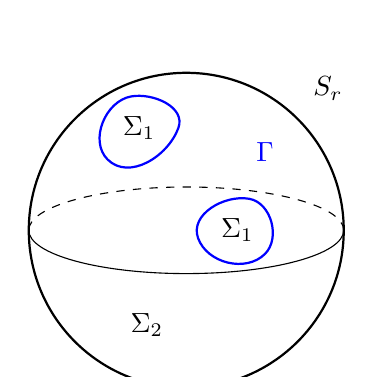
\begin{tikzpicture}
		%\draw[help lines] (-3,-3) grid (3,3);
		\draw [thick] (0,0) circle (2);
		\draw (-2,0) arc (180:360: 2 and 0.55);
		\draw [dashed] (2,0) arc (0:180: 2 and 0.55);
		
		\draw[thick, blue] (-1,.9) to[out=-45, in= 250] (-.1,1.3) to[out=70,in=10] (-.7,1.7) to [out=190, in=135](-1,.9);
		\draw[thick, blue] (1,-.3) to[out=-135, in= 290] (.15,-.1) to[out=110,in=170] (.8,.4) to [out=350, in=45](1,-.3);
		
		\node at (1.8,1.8) {\(S_r\)};
		\node at (-.6,1.3) {\(\Sigma_1\)};
		\node at (.65,0) {\(\Sigma_1\)};
		\node at (-.5,-1.2) {\(\Sigma_2\)};
		\node[blue] at (1,1) {\(\Gamma\)};
		\end{tikzpicture}
        \caption{Construction of the competitors \(\Sigma_1\) and \(\Sigma_2\).}
        \label{fig: connected components}
	\end{figure}
    Moreover,
    \[
		(n+1)\omega_{n+1}r^n = \Haus^n(S_r) = \Haus^n(\Sigma_1) + \Haus^n(\Sigma_2).
	\]
	Since \(\Sigma\) is area minimizing and \(\de (\Sigma \cap B_r)=\Gamma=\de \Sigma_1=\de \Sigma_2\), we deduce that
	
	\[
	2 \Haus^n( \Sigma \cap B_r (0)) \leq \Haus^n(\Sigma_1) + \Haus^n(\Sigma_2) = (n+1)\omega_{n+1}r^{n}. \qedhere
	\]
\end{proof}

\subsection{Closure of area minimizing currents}

\begin{defn}
    An \emph{integer rectifiable \(k\)-current} \(T\) is an element of the topological dual of the space of smooth compactly supported \(k\)-forms of \(\R^{n+1}\) which admits a representation
    \[
        \langle T , \omega \rangle = \sum_{j=1}^\infty \theta_j \int_{K_j} \omega 
    \]
    where \(\theta_j \in \Z\) and \(K_j \subset \Sigma_j\) are closed subsets of oriented \(k\)-dimensional \(C^1\)-submanifolds \(\Sigma_j\) of \(\R^{n+1}\). The class of integral \(k\)-currents in \(\R^{n+1}\) is denoted by \(\mathcal{I}_k(\R^{n+1})\). 
    
    The \emph{support} of a current \(T \in \mathcal{D}_k(\R^{n+1})\) is the complement of the maximal open set \(A\) such that \(\langle T,\omega \rangle = 0\) for every \(\omega \in \mathcal{D}^k(\R^{n+1})\) with \(\spt(\omega) \subset A\). The \emph{mass measure} of \(T\) is defined by
    \[
    \begin{aligned}
        \|T\|(\Omega) &\coloneq \sup \left\{ \langle T,\omega \rangle \colon \omega \in \mathcal{D}^k(\R^{n+1}), \|\omega\|_\infty \le 1\right\}  &&\text{if }\Omega \subset \R^{n+1} \text{ open}, \\
        \|T\|(E) &\coloneq \inf\{ \mu_T(\Omega) \colon \Omega \supset E \text{ open}\}  &&\text{if }E\subset \R^{n+1} \text{ Borel}.
    \end{aligned}
    \]
    The \emph{boundary} of \(T\) is the \((k-1)\)-current \(\de T \in \mathcal{D}_{k-1}(\R^{n+1})\) defined by forcing Stokes' theorem:
    \[
        \langle \de T, \vp \rangle \coloneq \langle T , \dif \vp \rangle \qquad \forall \vp \in \mathcal{D}_{k-1}(\R^{n+1}).
    \]
\end{defn}

The integer rectifiable current generated by a \(C^1\)-submanifold \(\Sigma\) is denoted by \(\llbracket \Sigma \rrbracket\).

Integer rectifiable currents are endowed with the weak* topology of Radon measures, i.e., if \(T_j, T \in \mathcal{I}_k(\R^{n+1})\), we say that \(T_j \weakstarto T\) if 
\[
    \langle T_j, \omega \rangle \to \langle T,\omega \rangle \qquad \forall\omega \in \mathcal{D}^k(\R^{n+1}).
\]

It holds the following compactness result (cf \cite[Chapter~6]{Simon_GMT1983})
\begin{thm}[Compactness, Federer-Fleming]
    If \((T_j)_j \subset \mathcal{I}_k(\R^{n+1})\) is such that for every \(\Omega \subset \subset \R^{n+1}\)
    \[
        \sup_j \mu_{T_j}(\Omega) + \mu_{\de T_j}(\Omega) < \infty,
    \]
    then \(T_j\) admits a weak* converging subsequence in \(\mathcal{I}_k(\R^{n+1})\).
\end{thm}

\begin{defn}
    An integral current \(T \in \mathcal{I}_n(\R^{n+1})\) is \emph{area minimizing} if for every \(\Omega \subset \subset \R^{n+1}\) and \(S \in \mathcal{I}_n(\R^{n+1})\) such that \(\de S=\de T\) and \(\spt(T-S) \subset \Omega\),
    \[
        \mu_T(\Omega) \le \mu_S(\Omega).
    \]
\end{defn}

Clearly, if \(\Sigma\) is an area minimizing hypersurface, the corresponding current \(\llbracket \Sigma \rrbracket\) is area minimizing as well.

Since \(T_j \weakstarto T\) implies that \(\de T_j \weakstarto \de T\) and \(\|T_j\| \weakstarto \|T\|\), the lower semicontinuity on open sets implies the following.
\begin{prop}[Closure of area minimizing currents]\label{prop: closure of area minimizing currents}
    If \(T_j \weakstarto T\) in \(\mathcal{I}_n(\R^{n+1})\) and each \(T_j\) is area minimizing with same boundary, then \(T\) is also area minimizing.
\end{prop}

\begin{defn}
    Let \(\phi \colon \R^{n+1} \to \R^{n+1}\) be a \(C^1\)-diffeomorphism and \(T \in \mathcal{I}_k(\R^{n+1})\). The \emph{push-forward}  of \(T\) along \(\phi\) is the integral current \(\phi_\#T\) defined by
    \[
        \langle \phi_\#T, \omega \rangle = \langle T, \phi^*\omega \rangle \qquad \forall \omega \in \mathcal{D}^k(\R^{n+1}).
    \]

    A current \(T \in \mathcal{I}_n(\R^{n+1})\) is \emph{stationary} if for every smooth 1-parameter family of diffeomorphisms \(\phi \colon \R^{n+1} \times (-\eps,\eps) \to \R^{n+1}\) with \(\phi_0 = \id\) and \(\phi|_{\R^{n+1}\setminus \Omega} = \phi_t|_{\R^{n+1}\setminus \Omega}\) for every \(t\) and some \(\Omega\subset \subset \R^{n+1}\) with \(\spt(\de T) \subset \R^{n+1}\setminus \Omega\),
    \[
        \left. \frac{\dif }{\dif t}\right|_{t=0} \|(\phi_t)_\#T\|(\Omega) = 0.
    \]
\end{defn}

\begin{rmk}
    An area-minimizing current is stationary.
\end{rmk}

\begin{defn}
    Given an integer rectifiable current \(T \in \mathcal{I}_n(\R^{n+1})\), a point \(x \in \spt(T)\) is a regular point of \(T\) if there exists \(r>0\) such that \(\spt(T) \cap B_r(x)\) is a smooth hypersurface of \(\R^{n+1}\). The set of regular points of \(T\) is denoted by \(\Reg(T)\) and \(\Sing(T) \coloneq \spt(T)\setminus \Reg(T)\) is the set of singular points of \(T\). The \emph{regularity scale} of \(T\) is the function \(r_T \colon \spt(T) \to [0,+\infty]\) defined as \(r_T(x)=0\) if \(x \in \Sing(T)\) and 
    \[
        r_T(x) \coloneq \sup \left\{ r>0 \colon \spt(T)\cap B_r(x) \text{ smooth hypersurface with }|A|^2\le r^{-1} \right\}
    \]
    if \(x \in \Reg(T)\). The set also
    \[
        \mathcal{R}_{\ge \rho} (T) \coloneq \{ x \in \spt(T) \colon r_T(x) \ge \rho\}
    \]
    for every \(\rho>0\).
\end{defn}

\subsection{The monotonicity formula}

\begin{thm}[Monotonicity formula]\label{thm: monotonicity formula}
    Let \(T\) be an area minimizing integer rectifiable \(n\)-current in \(\R^{n+1}\) with \(\de T=0\). Then for all \(0<s<r < \infty\),
    \begin{equation*}
        \frac{\|T\|(B_r(p))}{r^n} - \frac{\|T\|(B_s(p))}{s^n} = \int_{A(p,s,r)} \frac{|\nabla^\perp (x-p)|^2}{|x-p|^{n}} \ \dif \|T\|(x),
    \end{equation*}
    where \(A(p,s,r) = B(p,r) \setminus \overline{B(p,s)}\).

    In particular, denoting by \(\omega_n\) the Lebesgue measure of the Euclidean unit ball of \(\R^n\), the \emph{density function}
    \[
        \Theta_T(p,r) \coloneq \frac{\|T\|(B(p,r))}{\omega_n r^n}
    \]
    is non decreasing and it's constant if and only if \(T\) is a cone with vertex \(p\), i.e., \((\eta_{p,\lambda})_\# T = (\eta_{p,0})_\#T\) for every \(\lambda>0\).
\end{thm}

The monotonicity formula does not depend on the orientation, and in fact it extends in the larger class of \emph{stationary varifolds}. The idea of the proof is to test the radial vector field \(X(x)=x-p\) in the first variation formula. For the details see \cite[Chapter~8,\S3]{Simon_GMT1983}.

\section{The logarithmic cutoff trick for \texorpdfstring{$n=2$}{n=2}}
\begin{thm}[Bernstein]\label{thm: Bernstein}
	All entire solutions \(u \colon \R^2 \to \R\) of \eqref{eq: MSE} are affine.
\end{thm}
\begin{proof}
	Let \(\Sigma = \gr(u)\). 
	The idea is to plug \(f=1\) into \eqref{eq: stability inequality} to prove that \(|A_\Sigma|^2=0\), which implies that the Gauss map is constant. However, we actually need to approximate it by compactly supported functions that we can test in \eqref{eq: stability inequality}. To do so, we can use a logarithmic cutoff trick: for any \(k \in \N\), let \(f_k \colon \R^3 \to \R\) be defined by (up to smoothing)
	\[
		f_k(x) \coloneq \begin{cases}
			1 &\text{if }|x| \leq e^k \\
			2- \frac{\log |x|}{\log R} &\text{if }e^k< |x| \leq e^{2k} \\
			0 &\text{if }|x| > e^{2k}
		\end{cases}
	\]
	Then, if \(r=|x|\) is the distance from the origin
	\[
		|\nabla_\Sigma f_k| \leq |\nabla f_k | = \frac{1}{k r} \qquad e^k \leq r \leq e^{2k}.
	\]
	Now one would like to integrate in spherical coordinates and then estimate. Recall that by Theorem~\ref{thm: quadratic area growth for entire minimal graphs}, 
	\[
		\Area(\Sigma \cap B_r) \leq 2\pi r^2 \qquad \forall r>0.
	\]
	Moreover, since for all \(k+1 \leq \ell \leq 2k\), if \(A_\ell = A(e^\ell,e^{\ell-1}) =B_{e^\ell} \setminus B_{e^{\ell-1}} \)
	\[
		\sup_{A_\ell \cap \Sigma} |\nabla_\Sigma f_k|^2 \leq \frac{1}{k^2 e^{2\ell-2}}.
	\]
	Then we can estimate
    \begin{equation}\label{eq: Bernstein estimate}
	\begin{aligned}
		\int_\Sigma |\nabla_\Sigma f|^2 &\leq \sum_{\ell=k+1}^{2k} \int_{A_\ell \cap \Sigma} |\nabla_\Sigma f|^2 \\
		&\leq \sum_{\ell=k+1}^{2k} \frac{\Area(B_{e^\ell} \cap \Sigma)}{k^2 e^{2\ell-2}} \\
		&\leq \frac{2\pi e^2}{k} \longrightarrow 0.
	\end{aligned}
    \end{equation}
	Then the second fundamental form \(A_\Sigma \equiv 0\), and so the unit normal is constant. This means that \(\Sigma\) is planar, hence \(u\) an affine function.
\end{proof}

This proof cannot work in higher dimension, because the \emph{quadratic} extrinsic volume growth estimate is crucial. 

\section{Area minimizing cones}
For every \(p \in \R^{n+1}\) and \(\lambda>0\), let
\[
    \eta_{p,\lambda}(x) = \frac{x-p}{\lambda} \qquad \forall x \in \R^{n+1}.
\]

\begin{defn}
    A \emph{cone} in \(\R^{n+1}\) with vertex \(p \in \R^{n+1}\) is a subset \(C \subseteq \R^{n+1}\) such that
    \[
     \eta_{p,\lambda}(C)=\eta_{p,0}(C) \qquad \forall \lambda>0.
    \]
    The \emph{link} of a cone \(C\) is
    \[
        S=S(C) \coloneq C \cap \Sp^{n}(p),
    \]
    where \(\Sp^{n}(p)\) is the unit sphere centered at \(p\).
\end{defn}

From now on, unless explicitly specified, every cone is assumed to have vertex \(p=0\). For any \(r>0\), we will denote
\[
    C_r \colon \{ x \in C \colon 0<|x|<r \}, \qquad S_r = \{ x \in C \colon |x|=r\}.
\]

The \emph{regular set} \(\Reg(C)\) of the cone \(C\) is the maximal relatively open set \(M \subset C\) which is a smooth submanifold of \(\R^{n+1}\).The \emph{singular set} of \(C\) is \(\Sing(C) \coloneq C \setminus \Reg(C)\). A cone \(C\) is said to be \emph{regular} if \(\Sing(C) \subseteq \{p\}\).

\begin{rmk}
    If \(C \subset \R^{n+1}\) is a cone with link \(S\), then clearly
    \[
        C \setminus \{0\}= \bigcup_{v \in S}\{ tv \colon t>0 \}.
    \]
    Thus \(S\) is a smooth submanifold of \(\Sp^{n}\) if and only if \(C\) is a regular cone.
\end{rmk}

If \(\llbracket C \rrbracket\) is a stationary current, then \(\Reg(C)\) is a minimal hypersurface, as one can always take variations supported on \(\Reg(C)\). 

\subsection{Analysis of the Jacobi operator of a cone}
Let \(C \subset \R^{n+1}\) be an \(n\)-dimensional cone in the sense of currents (i.e., \(C\) is a current which is scale invariant). 

If \(r(x) = |x|\), then a simple computation is spherical coordinates show that on \(\Reg(C)\)
\begin{equation*}
    \begin{aligned}
        g_C &= \dif r^2 + r^2 g_S,\\
        A_C &= r^{-1}A_S, \\
        \Delta_C &= \frac{\de^2}{\de r^2} + \frac{n-1}{r} \frac{\de}{\de r} + \frac{1}{r^2} \Delta_S
    \end{aligned}
\end{equation*}
where \(A_S\) is the second fundamental form of (the regular part of) \(S\) in \(\Sp^n\). As a consequence:
\begin{prop}\label{prop: cone minimal iff link minimal}
    A regular cone \(C \subset \R^{n+1}\) is minimal if and only if its link \(S\) is a minimal submanifold of \(\Sp^{n}\).
\end{prop}

Let \(C \subset \R^{n+1}\) be a regular \(n\)-dimensional minimal cone (or also the regular part of a stationary cone, e.g. \(\mathcal{R}_{\ge \rho}(C)\) for some \(\rho>0\)). Its Jacobi operator is
\[
L_C = \frac{\de^2}{\de r^2} + \frac{n}{r} \frac{\de}{\de r} + \frac{1}{r^2} (\Delta_S +|A_S|^2).
\]
We will study independently the two operators
\[
    L = \Delta_S +|A_S|^2
\]
on the link and 
\[
    P=r^2 \frac{\dif^2}{\dif r^2} + (n-1)r \frac{\dif }{\dif r}
\]
on a segment, and then combine the obtained results. 

Consider \(L \coloneq \Delta_S + |A_S|^2\) on a relatively open subset \(\Omega\) of \(S\) with smooth (possibly empty, if \(S\) is smooth) boundary, and impose homogeneous Dirichlet conditions. By standard elliptic theory, it can be diagonalized, i.e., we can find a Hilbert basis \(\{\psi_j\}_{j \in \N}\) of \(C^\infty_0(\Omega)\) and a monotone sequence
\[
    \mu_1 \le \mu_2 \le \dots  \to \infty
\]
such that
\[
    -L\psi_j = \mu_j \psi_j.
\]
Moreover,
\begin{equation}\label{eq: variational eigenvalue}
    \mu_1 = \mu_1(\Omega) = \inf \left\{ \frac{\int_\Omega |\nabla u|^2- |A_S|^2u^2}{\int_\Omega u^2} \colon u \in C^\infty_c(\Omega) \setminus \{0\}\right\}.
\end{equation}

\begin{lemma}\label{lemma: 1st eigenvalue of minimal hypersurfaces in the sphere}
    Let \(S \subset \Sp^n\) be a closed (i.e. compact and without boundary) minimal hypersurface of the round \(n\)-sphere. If \(S\) is not a totally geodesic \((n-1)\)-sphere, then
    \[
        \mu_1(S) \le -(n-1).
    \]
\end{lemma}
\begin{proof}
    Test the function \(u= |A_S|\) (up to smoothing) and use Simons' identity \cite[Theorem~5.3.1]{Simons_MinimalVarieties1968}:
    \begin{equation}\label{eq: Simons identity}
        \Delta_S A_S = (n-1-|A_S|^2)A_S.
    \end{equation}

    Fix an orthonormal frame \(E_1,\dots,E_{n-1}\) tangent to \(S\). Observe that
    \[
        \nabla_X |A_S| = |A_S|^{-1}\langle \nabla_X A_S, A_S \rangle 
    \]
    for any \(X \in \VF(S)\), so
    \[
    \begin{split}
        \nabla_{E_i} (\nabla_{E_i}|A_S|) &= -|A_S|^{-3} \langle \nabla_{E_i} A_S, A_S \rangle^2 + |A_S|^{-1}(|\nabla_{E_i}A_S|^2+ \langle \nabla_{E_i} \nabla_{E_i} A_S, A_S \rangle ) \\
        \nabla_{\nabla_{E_i}E_i} |A_S| &= |A_S|^{-1}\langle \nabla_{\nabla_{E_i}E_i} A_S, A_S \rangle.
    \end{split}
    \]

    Then,
    \begin{align*}
        \Delta_S |A_S| &= \sum_i \nabla_{E_i} (\nabla_{E_i} A_S) - \sum_i \nabla_{\nabla_{E_i}E_i}A_S \\
        &= |A_S|^{-1} \sum_i \langle \nabla_{E_i}\nabla_{E_i} A_S - \nabla_{\nabla_{E_i}E_i} A_S, A_S \rangle \\
        &\qquad \qquad \qquad + |A_S|^{-1} \sum_i (|\nabla_{E_i}A_S|^2 - |A_S|^{-2}\langle\nabla_{E_i}A_S, A_S \rangle ^2 ).
    \end{align*}
    By Cauchy-Schwarz inequality,
    \begin{align*}
        |\nabla_{E_i}A_S|^2 - |A_S|^{-2}\langle\nabla_{E_i}A_S, A_S \rangle^2 &\ge |\nabla_{E_i}A_S|^2 - |\nabla_{E_i}A_S|^2 \ge 0.
    \end{align*}
    By \eqref{eq: Simons identity},
    \begin{align*}
        \Delta_S |A_S| &\ge |A_S|^{-1} \sum_i \langle \nabla_{E_i}\nabla_{E_i} A_S - \nabla_{\nabla_{E_i}E_i} A_S, A_S \rangle = |A_S|^{-1}{\langle \Delta A_S,A_S\rangle} \\
        &= (n-1-|A_S|^2)|A_S|.
    \end{align*}

    Testing \(u=|A_S|\) (up to smoothing) in \eqref{eq: variational eigenvalue} we get
    \begin{align*}
        \mu_1 &\le \frac{1}{\int_S |A_S|^2\dif \sigma}\int_S |\nabla_S |A_S||^2 \dif \sigma - \int_S |A_S|^4\dif \sigma \\
        &= -\frac{1}{\int_S |A_S|^2 \dif \sigma} \int_S |A_S| \Delta |A_S| +|A_S|^4 \dif \sigma \\
        &\le -\frac{1}{\int_S |A_S|^2 \dif \sigma} \int_S (n-1) |A_S|^2 \dif \sigma \\
        &= -(n-1). \qedhere
    \end{align*}
\end{proof}

\begin{rmk}\label{rmk: 1st eigenvalue on the link}
    If \(C\) is not regular, then there exists \(\rho_0>0\) such that
    \[
        \mu_1(\mathcal{R}_{\ge \rho_0}\cap \Sp^n) \le -(n-1).
    \]
    The idea is again to test \(u=|A_S|\), but of course one needs to be even more careful because \(|A_S|\) does not vanish at \(\de (\mathcal{R}_{\ge \rho_0}\cap \Sp^n)\). 
\end{rmk}

Let us now consider the differential operator
\[
    Pu (r)= r^2 u''(r) + (n-1)r u'(r).
\]
Given \(\mu \in \R\), we can find a general (complex) solution of 
\[
    Pu =\mu u
\]
by plugging the ansatz \(u(r)=r^\gamma\), getting that
\[
    \gamma^2+(n-2)\gamma =\mu
\]
so
\[
    \gamma = \gamma^\pm(\mu) = \frac{2-n}{2} \pm \sqrt{ \left(\frac{n-2}{2}\right)^2 + \mu}.
\]

    \begin{figure}[ht]
        \centering
        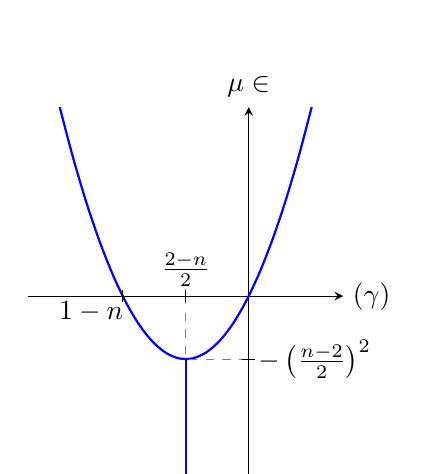
\begin{tikzpicture}[scale=0.8,>=stealth]
          % parameter
          \def\n{4}
          \pgfmathsetmacro{\m}{.5*(2-\n)}
          \pgfmathsetmacro{\t}{\m*\m+(\n-2)*\m}
          \pgfmathsetmacro{\z}{2-\n}
          \pgfmathsetmacro{\a}{\m-2}
          \pgfmathsetmacro{\b}{\m+2}
          \pgfmathsetmacro{\f}{\b*\b+(\n-2)*\b}
        
          % axes
          \draw[->] (\a-0.5,0) -- (\b+0.5,0) node[right] {$\re(\gamma)$};
          \draw[->] (0,\t-2) -- (0,\f) node[above] {$\mu \in \R$};
        
          % parabola: lambda = gamma^2 + (n-2)*gamma + 1 - n, gamma real
          \draw[domain=\a:\b,samples=20,smooth,thick,blue]
            plot(\x,{\x*\x + (\n-2)*\x});

          % real trace: re(gamma) = (n-2)/2
          \draw[thick, blue](\m,\t)--(\m,\t-2);

        
          % labels
          \draw (\z,-.1)--(\z,.1);
          \node at (\z-.5,-.25) {$1-n$};

          \draw[dashed,gray] (\m,0) -- (\m,\t)--(0,\t);
          \draw (\m,.1)--(\m,-.1);
          \draw (-.1,\t)--(.1,\t);
          \node[above] at (\m,0){\(\frac{2-n}{2}\)};
          \node[right] at (0,\t){\(-\left(\frac{n-2}{2}\right)^2\)};        
        \end{tikzpicture}
        \caption{In blue \(\{(\re(\gamma),\mu) \in \R^2 \colon\gamma^2+(n-2)\gamma = \mu\}\).}
        \label{fig: parabola}
    \end{figure}

Substituting \(v=r^{-\gamma}u\) with \(\gamma = \gamma^\pm(\mu)\), we find that
\[
   \left[r^{n-1+2\gamma}v' \right]' = 0.
\]
Thus \(v' = cr^{1-n-2\gamma}\), so the general solution of \(Pu=\mu u\) (in \(\C\)) is 
\begin{equation}\label{eq: general solution of u}
u(r)= \left\{
\begin{aligned}
    &c_1 r^{2-n-\gamma} + c_2 r^\gamma &&\gamma \ne \frac{2-n}{2} \iff \mu \ne - \left(\frac{n-2}{2}\right)^2 \\
    &c_1 r^{\frac{2-n}{2}}(\log r + c_2) && \gamma = \frac{2-n}{2} \iff \mu = - \left(\frac{n-2}{2}\right)^2.
\end{aligned}\right.
\end{equation}
for some \(c_1,c_2 \in \C\). 

A direct computation shows that \(P\) is self-adjoint with respect to the scalar product
\[
    (u,v) \coloneq \int_a^b u(r)v(r)r^{n-3} \dif r,
\]
i.e., if \(u,v \in C^2_0([a,b])\),
\[
    \int_a^b vL_1u r^{n-3} \dif r = \int_a^b uL_1v r^{n-3}\dif r
\]
\begin{lemma}\label{lemma: eigenvalues of P}
    Given \(0<a<1<b<\infty\), the eigenvalues of \(P\) in \(H^1_0(a,b)\) are
    \begin{equation}\label{eq: spectrum of P}
            \delta_j^a = \left( \frac{n-2}{2} \right)^2 + \left( \frac{j\pi}{\log(a)} \right)^2, \qquad \delta_j^b = \left( \frac{n-2}{2} \right)^2 + \left( \frac{j\pi}{\log(b)} \right)^2
    \end{equation}
    Moreover, the respective eigenfunctions form a Hilbert basis of \(L^2(a,b)\) with respect to the scalar product
    \[
        (u,v) \coloneq \int_a^b u(r)v(r)r^{n-3} \dif r.
    \]
\end{lemma}
\begin{proof}
    Let \(u \colon (a,b) \to \C\) as in \eqref{eq: general solution of u} and look at its real and complex parts: assuming that \(c_1,c_2 \in \R\),
    \[
    \begin{aligned}
        \re(u(r)) &= \left(c_1 e^{(2-n-\re(\gamma))\log r} +c_2 e^{\re(\gamma)\log r}\right) \cos (\im(\gamma)\log r) \\
        \re(u(r)) &= \left(-c_1 e^{(2-n-\re(\gamma))\log r} +c_2 e^{\re(\gamma)\log r}\right) \sin (\im(\gamma)\log r)
    \end{aligned}
    \]
    Observe that if \(\im(\gamma)=0\), then \(\im(u) \equiv 0\) and imposing that \(\re(u(a))=\re(u(b))=0\) would imply that \(c_1=c_2=0\). Thus \(\im(\gamma)\ne 0\) and we have to choose \(\delta=-\mu\) so that \(\cos(\im(\gamma)\log r)\) or \(\sin(\im(\gamma)\log r)\) vanishes either at \(r=a\) or at \(r=b\). This implies that
    \[
        \delta = \left( \frac{n-2}{2} \right)^2 + \left( \frac{j\pi}{\log(a)} \right)^2 \quad \text{ or } \quad \delta = \left( \frac{n-2}{2} \right)^2 + \left( \frac{j\pi}{\log(b)} \right)^2
    \]
    for some integer \(j \ge 1\).
\end{proof}

\begin{thm}[Simons {\cite{Simons_MinimalVarieties1968}}]\label{thm: stability of cones}
    If \(C\subset \R^{n+1}\) is a regular \(n\)-dimensional minimal cone, then
    \[
        d_0(C) = \left(\frac{n-2}{2}\right)^2+\mu_1(S).
    \]
\end{thm}
\begin{proof}
    Let 
    \[
        \Omega_\eps \coloneq \{ rv \in C \colon v \in S, \ \eps < r < \eps^{-1}\}.
    \]
    
    Observe that, for every \(\Omega \subset \subset C\setminus\{0\}\), 
    \begin{align*}
        \lambda_1(\Omega) = \inf \left\{ -\frac{\int_{\Omega} \langle u, L_Cu \rangle \dif \mu_C}{\int_{\Omega} |u|^2\dif \mu_C} \ \colon \ u \in C^\infty_0(\Omega;N\Omega) \right\} \ge \lambda_1(\Omega_\eps)
    \end{align*}
    if \(\eps\) is small enough. Thus,
    \[
        d_0(C) = \lim_{\eps \downarrow 0} \lambda_1(\Omega_\eps),
    \]
    so we need to compute \(\lambda_1(\Omega_{\eps})\).

    Let \(\{\vp_i\}\) be the eigenfunctions of \(P\) in \(H^1_0(\eps,1/\eps)\), which form a Hilbert basis of \(L^2(\eps,1/\eps)\) with respect to the scalar product of Lemma~\ref{lemma: eigenvalues of P}. It's not hard to prove that the set spanned by \(\{\vp_i\psi_j\}_{i,j}\) is dense in \(C^0(\overline{\Omega_\eps})\), which is dense in \(L^2(\Omega_\eps)\), so 
    \[
        \overline{\Span(\{\vp_i\psi_j\}_{i,j})}^{L^2} = L^2(\Omega_\eps).
    \]
    Moreover,
    \[
        \int_{\Omega_\eps} \vp_i \psi_j\vp_k \psi_l  r^{-2}\dif \mu_C = \int_\eps^{1/\eps} \vp_i \vp_k r^{n-3} \dif r \int_S \psi_j, \psi_l\dif \sigma = \delta_{ik} \delta_{jl}.
    \]
    Therefore, \(\{\vp_i\psi_j\}_{i,j}\) is a Hilbert basis of \(L^2(\Omega_\eps)\) with respect to the scalar product 
    \[
        (u,v) \coloneq \int_{\Omega_\eps} uv r^{-2}\dif \mu_C.
    \]
    Moreover,
    \begin{align*}
       -L_C \vp_i\psi_j &= -\frac{1}{r^2}P\vp_i \psi_j - \frac{1}{r^2}\vp_iL\psi_j \\
       &= r^{-2}(\lambda_i+\mu_j) \vp_i \psi_j,
    \end{align*}
    so, if \(u = \sum_{i,j}a_{ij}\vp_i \psi_j\), 
    \begin{align*}
        -\int_{\Omega_\eps} L_C X \vp_i \psi_j \dif \mu_C &= -\sum_{i,j,k,l} a_{ij}a_{kl}\int_{\Omega_\eps} -L_C \vp_i\psi_j \vp_k\psi_l \ \dif \mu_C \\
        &= \sum_{i,j,k,l} a_{ij}a_{kl}(\delta_i+\mu_j )\int_{\Omega_\eps} \vp_i\vp_k \psi_i\psi_l r^{-2} \dif \mu_C \\
        &= \sum_{i,j}a_{ij}^2(\delta_i+\mu_j).
    \end{align*}
    Therefore,
    \[
        \lambda_1(\Omega_\eps) = \delta_1 + \mu_1= \left( \frac{n-2}{2} \right)^2 + \left( \frac{j\pi}{\log \eps} \right)^2 + \mu_1.
    \]
    Now let \(\eps \downarrow 0\).
\end{proof}

\begin{thm}\label{thm: stability, n<7 => hyperplane}
    Let \(C \subset \R^{n+1}\) be a stable regular minimal \(n\)-dimensional cone. If \(n \le 6\), then \(C\) is a hyperplane.
\end{thm}
\begin{proof}
    Let \(C\) be a stable minimal cone. By Theorem~\ref{thm: stability of cones}, 
    \[
        \mu_1 \ge - \left( \frac{n-2}{2} \right)^2.
    \]
    Now, assume that \(S\) is not a totally geodesic hypersphere. By Lemma~\ref{lemma: 1st eigenvalue of minimal hypersurfaces in the sphere},
    \[
        \mu_1 \le -(n-1),
    \]
    so,
    \[
        (n-1) \le \left( \frac{n-2}{2} \right)^2,
    \]
    and this happens if and only if \(n \ge 7\).
\end{proof}

\subsection{Federer's dimension reduction argument}

\begin{thm}[Federer]\label{thm: Federer reduction}
    Let \(C \subset \R^{n+1}\) be an area minimizing cone and suppose that it's singular at least at two different points. Then there exists an area minimizing cone \(C'\subset \R^n\).
\end{thm}
\begin{proof}
    Let \(x_0 \in \Sing(C) \setminus \{0\}\). By scaling invariance, then all the half line \(\{tx_0 \colon t>0\} \subset \Sing(C)\), so we can also assume that \(x_0 \in \Sp^n\). The monotonicity formula implies that 
    \[
        \Theta_C(x_0) = \lim_{r \to 0}\Theta_F(x_0,r) 
    \]
    exists and is finite. Let \(\lambda_h \to 0\) and consider \(C_h = (\eta_{x_0,\lambda_h})_\#\llbracket C \rrbracket \). By the monotonicity formula, for every \(r>0\)
    \[
        \|C_h\|(B_r) = \omega_n\Theta_C(x_0,\lambda_hr) \to \Theta_C(x_0),
    \]
    so by weak* compactness, up to a subsequence, \(C_h \weakstarto T\) in \(\mathcal{I}_n(\R^{n+1})\). By the closure of area minimizing currents, \(T\) is area minimizing. Since \(\|C_h\| \weakstarto \|T\|\) as measures, by lower semicontinuity on open sets and upper semicontinuity on compact sets
    \[
        \|C_h\|(B_r) \to \|T\|(B_r)
    \]
    for every \(r>0\) such that \(\de B_r \cap \left( \spt \|T\| \cup \bigcup_h\spt\|C_h\| \right) = \varnothing\), i.e., for all \(r>0\) except for at most countable set. Thus
    \[
        \Theta_T(0,r) = \lim_{h \to \infty} \Theta_{C_h}(0,r) = \Theta_C(x_0),
    \]
    so by the rigidity statement of Theorem~\ref{thm: monotonicity formula} \(T=\llbracket C''\rrbracket\) is a cone with vertex 0 (regular points have density one). Since every dilation centered at 0 look like a translation in the \(x_0\)-direction near \(x_0\), \(C''\) is invariant under translations in the \(x_0\)-direction, hence, up to a rotation, \(C''=C'\times \R\) for some cone \(C'\subset \R^n\). We conclude by noticing that \(C''=C' \times \R\) is area minimizing in \(\R^{n+1}\) if and only if \(C'\) is area minimizing in \(\R^n\).
\end{proof}

\begin{cor}\label{cor: every area minimizing cone is flat for n<8}
    If \(n+1\le 7\), every area minimizing \(n\)-dimensional cone in \(\R^{n+1}\) is a hyperplane. 
\end{cor}
\begin{proof}
    Suppose that \(C\) is a non-flat area minimizing \(n\)-cone in \(\R^{n+1}\). By Theorem~\ref{thm: stability, n<7 => hyperplane}, \(C\) has at least two singular points. By Federer's reduction argument, there exists a non-flat area minimizing \((n-1)\)-cone also in \(\R^n\). Proceeding like this, we would prove that there exists an area minimizing non-flat \(1\)-cone \(C' \subset \R^2\). But these are just unions of half-lines, and clearly they don't minimize the area(=length) unless they form a single line, as shown in Figure~\ref{fig: non area minimizing cones}.
\end{proof}
\begin{figure}[ht]
        \centering
        \begin{tikzpicture}
            \draw[thick] (0,0) -- (3,0);
            \draw[thick] (0,0) -- ({3*cos(40)},{3*sin(40)});
            \draw[red,thick] (1,0) -- ({cos(40)},{sin(40)});
        \end{tikzpicture}
        \caption{Unions of half-lines from the origin are not length minimizing.}
        \label{fig: non area minimizing cones}
\end{figure}

\begin{cor}\label{cor: dim(Sing(C)) <= n-7}
    If \(C \subset \R^{n+1}\) is an area minimizing \(n\)-dimensional cone, then \(\dim_\Haus(\Sing(C) \le n-7\).
\end{cor}
\begin{proof}
    Applying iteratively Theorem~\ref{thm: Federer reduction}, for every \(k \le \dim_\Haus(\Sing(C))\) we find an area-minimizing \((n-k)\)-cone \(C_k \subset \R^{n-k+1}\) with at least a singular point. But by Corollary~\ref{cor: every area minimizing cone is flat for n<8}, we know that we must stop before getting to \(\R^7\).
\end{proof}

\subsection{Existence of non-flat area minimizing cones}

In \cite{Simons_MinimalVarieties1968}, Simons introduced the famous \emph{Simons cone}
\[
    C_S \coloneq \{ (x,y) \in \R^4 \times \R^4 \colon |x|=|y|\} \subset \R^8,
\]
and he proved that it's stable (because the link is \(S=\Sp^3(1/\sqrt{2}) \times \Sp^3(1/\sqrt{2})\), and \(\mu_1(S)=-(n-1)=6\), so \(d_0(C)\ge 0\). One year later, Bombieri, De Giorgi and Giusti proved the following. 

\begin{thm}[Bombieri, De Giorgi, Giusti, {\cite{BombieriDeGiorgiGiusti_MinimalCones1969}}]\label{thm: C_S is area minimizing}
    \(\R^8 \setminus C_S\) is foliated by complete, smooth, area minimizing hypersurfaces \(\Sigma_\lambda\) (for \(\lambda \ne 0\)) which are invariant under the action of \(O(4)\times O(4)\) and such that \(\llbracket \Sigma_\lambda \rrbracket \weakstarto \llbracket C_S\rrbracket\) as \(\lambda \to 0\). In particular, \(C_S\) is area minimizing, and therefore \(C_S \times \R^{n-7} \subset \R^{n+1}\) is area minimizing for every \(n\ge 7\).
\end{thm}


\section{Solution to Bernstein problem}

\subsection{Tangent cones at infinity}
In this section, given a complete area minimizing hypersurface \(\Sigma \subset \R^{n+1}\), we construct ‘‘tangent cones at infinity'' by a \emph{blow down} procedure.

\begin{cor}[Existence of the tangent cone at infinity]\label{cor: existence of tangent cone at infinity}
    If \(\Sigma \subset \R^{n+1}\) is an area minimizing hypersurface, then there exists a sequence \(\lambda_h \to \infty\) and an area minimizing cone \(C\) such that \((\eta_{0,\lambda_h})_\#\llbracket\Sigma\rrbracket \weakstarto  C\).
\end{cor}
\begin{proof}
    By the extrinsic volume growth estimate of Theorem~\ref{thm: quadratic area growth for entire minimal graphs}, for every \(r>0\)
    \[
        \|\Sigma\|(B_r) =  \Haus^n(\Sigma \cap B_r) \le \frac{(n+1) \omega_{n+1}}{2} r^n,
    \]
    hence
    \[
        \Theta_\Sigma(\infty) \coloneq \lim_{r \to \infty}\Theta_\Sigma(0,r) < \infty.
    \]
    Fix a sequence \(\lambda_h \to \infty\) and let \(T_h = (\eta_{0,\lambda})_\#\llbracket\Sigma \rrbracket\). Since
    \[
        \|T_h\|(B_r) = \Haus^n((\lambda_h^{-1}\Sigma) \cap B_r) = \lambda_h^{-n}\Haus^n(\Sigma \cap B_{\lambda_hr})
    \]
    and \(\de T_h=0\), for every \(r>0\)
    \[
        \|T_h\|(B_r) \le \Theta_\Sigma(\infty)\omega_n r^n,
    \]
    so by weak* compactness there exists \(C \in \mathcal{I}_n(\R^{n+1})\) such that up to a subsequence \(T_h \weakstarto C\). By the closure of area minimizing currents, \(T\) is area minimizing. Since \(\|T_h\| \weakstarto \|C\|\) as measures, by lower semicontinuity on open sets and upper semicontinuity on compact sets
    \[
        \|T_h\|(B_r) \to \|C\|(B_r)
    \]
    for every \(r>0\) such that \(\de B_r \cap \left( \spt \|C\| \cup \bigcup_h\spt\|T_h\| \right) = \varnothing\), i.e., for all \(r>0\) except for at most countable set. Thus
    \[
        \Theta_C(0,r) = \lim_{h \to \infty} \Theta_{T_h}(0,r) = \lim_{h \to \infty} \frac{\Haus^n(\Sigma \cap B_{\lambda_hr})}{\omega_n \lambda_h^n r^n} = \Theta_\Sigma(\infty),
    \]
    so by the rigidity statement of Theorem~\ref{thm: monotonicity formula} \(T\) is a cone with vertex 0.
\end{proof}

\begin{defn}
    A cone \(C\) as in Corollary~\ref{cor: existence of tangent cone at infinity} is called a \emph{tangent cone at infinity} of \(\Sigma\).
\end{defn}


\subsection{A weaker Bernstein problem}

\begin{thm}\label{thm: Bernstein for area minimizing}
    Let \(\Sigma \subset \R^{n+1}\) be a complete area minimizing hypersurface. If \(n+1 \le 7\), then \(\Sigma\) is a hyperplane.
\end{thm}
\begin{proof}
    Let \(C\) be a tangent cone at infinity, and observe that \(\Theta_C \equiv \Theta_\Sigma(\infty)\). By Corollary~\ref{cor: every area minimizing cone is flat for n<8}, \(C\) is a hyperplane, so \(\Theta_C \equiv 1\). Then by the monotonicity formula (assuming without loss of generality that \(0 \in \Sigma\))
    \[
        1=\lim_{r \to 0^+}\Theta_\Sigma(0,r) \le \Theta_\Sigma(\infty)=\Theta_C=1,
    \]
    so \(\Theta_\Sigma \equiv 1\). The rigidity case of the monotonicity formula implies that \(\Sigma\) is a cone, so \(\Sigma = C\) is a hyperplane.
\end{proof}

Since minimal graphs are calibrated, this implies that if \(u \colon \R^n \to \R\) solves \eqref{eq: MSE} and \(n \le 6\), then \(u\) is affine. 

For every \(n+1\ge 8\), Theorem~\ref{thm: C_S is area minimizing} yields counterexamples. 

\subsection{The ‘‘cone version'' of the Bernstein problem}
Recall also the following.
\begin{thm}[Strong maximum principle for minimal hypersurfaces]
    Let \(\Sigma_1\) and \(\Sigma_2\) be minimal hypersurfaces in \(\R^{n+1}\) and suppose that there exists an open set \(\Omega \subset \R^{n+1}\) such that \(\Sigma_1\) separates \(\Omega\) in two connected components and \(\Sigma_2\) lies in the closure one of them. If \(\Sigma_2\cap\Sigma_1\cap \Omega\ne \varnothing\), then \(\Sigma_2\cap\Omega \subset \Sigma_1\).
\end{thm}
\begin{proof}
    Expressing \(\Sigma_1\) and \(\Sigma_2\) as graphs of functions \(u_1\le u_2\) locally, then \(u_1\) and \(u_2\) solve \(\eqref{eq: MSE}\) \(v = u_2-u_1 \ge 0\) solves the second order elliptic PDE
    \[
        \dive(A\nabla v) = 0,
    \]
    where 
    \[
        A(x) = \int_0^1 \frac{\nabla u_1(x) + t\nabla u_2(x)}{\sqrt{1+|\nabla u_1(x) + t\nabla u_2(x)|^2}} \dif t,
    \]
    so the strong maximum implies that either \(v>0\) or \(v \equiv 0\). If \(\Sigma_1\) and \(\Sigma_2\) touch, \(v\equiv0\) and with an obvious connectedness argument we get that \(\Sigma_2 \cap \Omega \subset \Sigma_1\).
\end{proof}

\begin{thm}[De Giorgi]\label{thm: De Giorgi splitting}
    Let \(u \colon \R^n \to \R\) be an entire solution of \eqref{eq: MSE}. Then any tangent cone at infinity of \(\gr(u)\) splits as \(C'\times \R\).
\end{thm}
\begin{proof}
    Let \(\Sigma=\gr(u)\). Since it's a graph, every tangent cone at infinity has density 1 at almost every point, so every tangent cone at infinity is of the form \(\llbracket C\rrbracket\) for some cone \(C\) with vertex 0. Fix one and let \(\lambda_k \to \infty\) such that \((\eta_{0,\lambda_k})_\# \llbracket\Sigma\rrbracket \weakstarto \llbracket C \rrbracket\).

    Since \(\Sigma\) is a graph, \(\Sigma + \lambda_k e_{n+1}\) is disjoint from \(\Sigma\), so \(C\) lies on one side of \(C+e_{n+1}\). The strong maximum principle for minimal hypersurfaces (applied to the regular part of \(C\), which is open and dense in \(C\)) implies that either \(C=C+e_{n+1}\) or \(C\) and \(C+e_{n+1}\) are disjoint. In the first case, we conclude that \(C\) is invariant under translations in the \(e_{n+1}\)-direction, so \(C=C'\times \R\). In the second case, we apply Theorem~\ref{thm: Bernstein for cones} to conclude that \(C\) is a hyperplane.
\end{proof}



\begin{thm}\label{thm: Bernstein for cones}
    If \(C\) is an area minimizing \(n\)-cone in \(\R^{n+1}\) that is disjoint from \(C+e_{n+1}\), then \(C\) is a hyperplane.
\end{thm}

This is a sort of Bernstein problem for cones. Indeed, by scaling invariance, saying that \(C\) is disjoint from \(C+e_{n+1}\) is like saying that the family \(C+\lambda e_{n+1}\) for \(\lambda \in \R\) is disjoint, and this is a weaker notion of being a graph. For solving Bernstein problem we only need \(n=7\), and in this way by Corollary~\ref{cor: dim(Sing(C)) <= n-7} \(C\) is regular. For the general case one can use a more refined argument together with Remark~\ref{rmk: 1st eigenvalue on the link}.

\begin{proof}[Proof for \(n=7\)]
    by Corollary~\ref{cor: dim(Sing(C)) <= n-7} \(C\) is regular. Let \(\nu_S\) be a unit normal of the link \(S\) in \(\Sp^n\) and note that \(\nu(rv) \coloneq \nu_S(v)\) defines a unit normal of \(C\). The function \(u = \nu \cdot e_{n+1}\) is the Jacobi field generated by moving \(C\) along the \(e_{n+1}\)-direction. Moreover, up to choose the right unit normal, \(u \ge 0\) in a (punctured) neighborhood of 0, so \(u\ge 0\) everywhere. Since \(u\) does not depend on \(r\), 
    \[
        0= r^2L_Cu = \Delta_S u + |A_S|^2u=Lu,
    \]
    and the strong maximum principle implies that \(u>0\) everywhere.
    Let \(\psi_1>0\) be an eigenfunction of \(L\) associated to \(\mu_1=\mu_1(S)\) (which can always be chosen with a sign). Then
    \[
        0 = \int_S Lu \psi_1 = \int_S u L\psi_1  = -\mu_1 \int_S u\psi_1, 
    \]
    so \(\mu_1=0\). But this happens if and only if \(S\) is a totally geodesic hypersphere of \(\Sp^n\), so \(C\) is a hyperplane.
\end{proof}

\subsection{Solution of the Bernstein problem}

Let \(u \colon \R^n \to \R\) solve \eqref{eq: MSE} and \(\Sigma = \gr(u)\). Let \(C\) be a tangent cone at infinity of \(\Sigma\). By Theorem~\ref{thm: De Giorgi splitting}, \(C= C' \times \R\) for some other area minimizing cone \(C' \subset \R^n\). 

If \(n\le 7\), then \(C' \cong \R^{n-1}\) is a hyperplane in \(\R^n\), so \(C \cong \R^n\) is a hyperplane in \(\R^{n+1}\). Then, as in the proof of Theorem~\ref{thm: Bernstein for area minimizing}, \(\Theta_\Sigma \equiv \Theta_C \equiv 1\), so \(\Sigma = C\) is a hyperplane.

If \(n \ge 8\), Bombieri, De Giorgi and Giusti in \cite{BombieriDeGiorgiGiusti_MinimalCones1969} constructed a function \(u \colon \R^n \to \R\) solving \eqref{eq: MSE} and such that its graph has \(C_S \times \R^{n-8} \times \R\) as a tangent cone at infinity.

\printbibliography
\end{document}

